\documentclass{article}
\usepackage[utf8]{inputenc}
\usepackage[T1]{fontenc}
\usepackage{amsmath}
\usepackage{hyperref}
\usepackage{graphicx}
\usepackage{url}
\usepackage{subfigure}

\newcommand{\code}{\texttt}

\title{Project in Information-Theoretic Modeling Final Report}
\author{Aleksi Hartikainen \and Mikko Sysikaski}

\begin{document}
\maketitle

%\abstract{}

%\newpage
%\tableofcontents
%\newpage

\section{Problem 1}

The first task was to compress a sequence of bits using side data that was also available during decompression.

The file to be compressed had $100\,000$ binary digits, so trivially packing the bits yields a file of size $12\,500$ bytes.
For comparison, we also tried packing the data this way as the decompression code becomes much smaller and simpler.
This gave a total size of around 13.5~KiB uncompressed, and 12.5~KiB after compressing with gzip.

The task was to use arithmetic coding with probabilities from the given model.
Instead of using probabilities from model definition, we computed actual conditional frequencies from the data.
That is, for every tuple $(x_1,x_2,x_3,x_4)$ we counted how many times $x_0$ is 0 and 1, and this gave us the conditional probability of $x_0$ with respect to the other variables.
The calculated probabilities are shown in Figure~\ref{ex1_probs}.
We created a custom implementation of arithmetic coding that used the conditional probabilities of Figure~\ref{ex1_probs} to encode each bit.

Using arithmetic coding and the conditional probabilities, we got the data compressed in 8100~bytes.
Together with the decompression program, this gave a total file size of 9832~bytes.

To evaluate the correctness of our arithmetic coding implementation, we calculated also the theoretical bound for data size using entropy coding.
According to probabilities in Figure~\ref{ex1_probs}, the total entropy of the input file is 64790.4~bits, which is 8098.8~bytes, so the result generated by our implementation is within 1 byte of the theoretical optimum.


\begin{figure}

\begin{center}
\begin{tabular}{|c|c|c|c|c|c|}
\hline
$x_1$ & $x_2$ & $x_3$ & $x_4$ & $P(x_0 = 0)$ & $P(x_0 = 1) $ \\ \hline
   0 & 0 & 0 & 0 & 0.74244 & 0.25756 \\ \hline
   1 & 0 & 0 & 0 & 0.180631 & 0.819369 \\ \hline
   0 & 1 & 0 & 0 & 0.122035 & 0.877965 \\ \hline
   1 & 1 & 0 & 0 & 0.595336 & 0.404664 \\ \hline
   0 & 0 & 1 & 0 & 0.507643 & 0.492357 \\ \hline
   1 & 0 & 1 & 0 & 0.072675 & 0.927325 \\ \hline
   0 & 1 & 1 & 0 & 0.0461351 & 0.953865 \\ \hline
   1 & 1 & 1 & 0 & 0.359641 & 0.640359 \\ \hline
   0 & 0 & 0 & 1 & 0.888336 & 0.111664 \\ \hline
   1 & 0 & 0 & 1 & 0.37004 & 0.62996 \\ \hline
   0 & 1 & 0 & 1 & 0.277587 & 0.722413 \\ \hline
   1 & 1 & 0 & 1 & 0.78809 & 0.21191 \\ \hline
   0 & 0 & 1 & 1 & 0.733648 & 0.266352 \\ \hline
   1 & 0 & 1 & 1 & 0.177577 & 0.822423 \\ \hline
   0 & 1 & 1 & 1 & 0.119161 & 0.880839 \\ \hline
   1 & 1 & 1 & 1 & 0.582299 & 0.417701 \\ \hline
\end{tabular}
\end{center}
\caption{Conditional probabilities used in exercise 1}
\label{ex1_probs}
\end{figure}

\section{Problem 2}

The second task was to compress data consisting of stock prices of four different stocks over 10121 days.
The data consisted of floating point values with two decimals.
As we didn't want to think about floating point accuracy issues, we simply converted the initial data to integers by multiplying the values by 100 and divided our final result again by 100 before outputting it.

All the prices were under 500 so they can be stored as 16-bit integers.
Thus a trivial storing the data without any proper compression gives a total size of about 81~KiB.

To find a good compression scheme, we initially tried plotting the data, as shown in Figure~\ref{fig:ex2o}.
As there was no immedient regularity to be seen, we tried seeing how the values change by taking the differences of adjacent values, shown in Figure~\ref{fig:ex2d}.
It can be seen that there are some large negative peaks, but otherwise the differences stay close to zero.
The same behavior can be observed for each of the stocks.

\begin{figure}
	\subfigure[Original data]{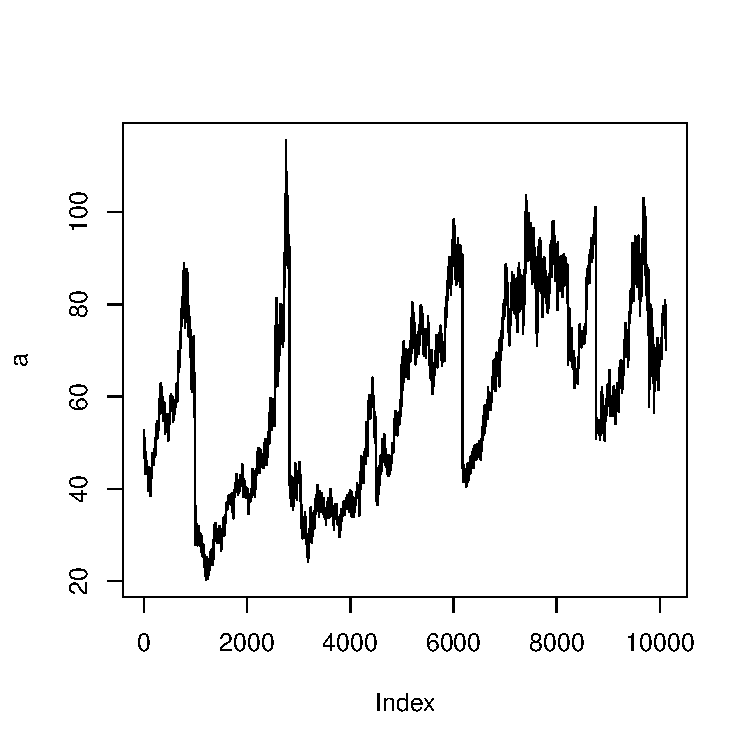
\includegraphics[scale=0.5]{ex2_orig.pdf}\label{fig:ex2o}}
	\subfigure[Differences of consecutive values]{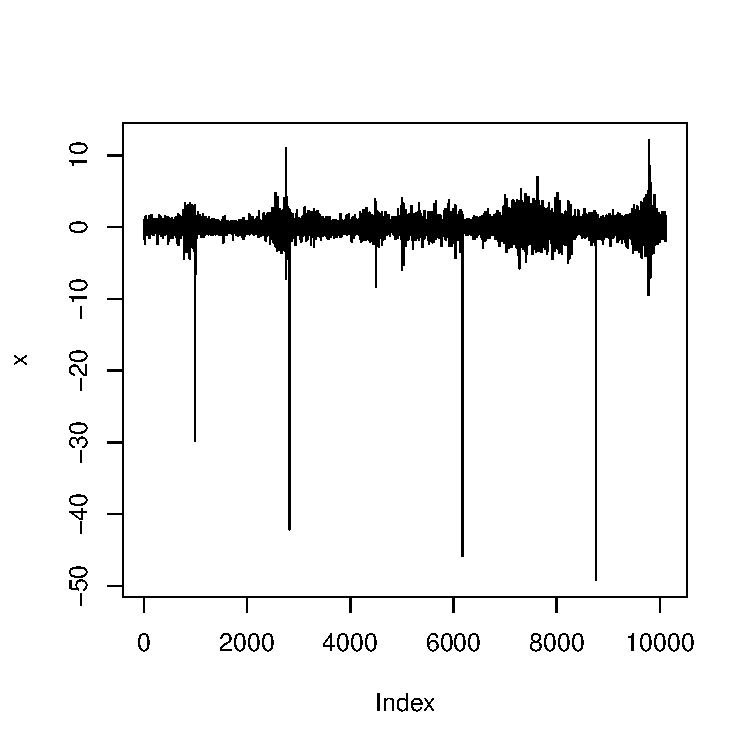
\includegraphics[scale=0.5]{ex2_diff.pdf}\label{fig:ex2d}}
	\caption{Plot of the first column of the data and the differences between its consecutive values. The original data shows a lot of irregularities, but except for a few peaks, the changes between consecutive values are quite small.}
\end{figure}

The connection between the four stocks changes didn't seem very simple so we decided to try simply compressing each of the stocks separately.
As our tests suggested that the differences between adjacent values are close to zero, we used a simple Gaussian model with mean equal to the previous value to calculate the probabilities for each value that where used in the arithmetic coding.

It seemed that the variance of the values varied quite a lot over time, so we used an adaptive scheme to decide the variance used by the normal distribution to compress each value.
The scheme works by maintaining a current approximation of variance $v_n$ and calculating new approximation $v_{n+1}$ each time we process a new value $x_{n+1}$.
The approximation is updated by taking weighted average using the formula $v_{n+1} = \frac{Lv_n + (x_{n+1}-x_n)^2}{L+1}$, where $L$ is a constant that decides how quickly the value changes.
We experimented with different values and saw that picking $L=10$ gives generally good results.

The Gaussian model with adaptive variance had a problem that the probability of the peaks is extremely low, around $10^{-100}$.
As our arithmetic coding uses 32-bit integers, it is impossible to cope with probabilities smaller than $2^{-30}$.
To fix this, we added a constant $2^{-30}$ to probabilities of all values and scaled the normal distribution probabilities so that the total probability still sums to 1.
As the largest number in the data (after converting to integers) was 45100, we only needed to add the constant to first 45101 integers, and scale the original probabilities by $\frac{2^{30}-45101}{2^{30}} \approx 0.999953$.
This factor is so close to 1 that it doesn't hinder the overall compression quality much, while adding the constant guarantees that any value can be encoded using no more than 30 bits.
We later noticed that increasing the constant further doesn't hinder the overall compression efficiency much, so we increased it to about $2^{20}$ and decreased the scaling factor accordingly, which saved some dozens of bytes in encoding the peak values.

Another improvement with regard to the peaks was to not update the variance when the value changed too much.
Updating the variance on peaks made encoding the values following it take significantly more space than necessary.
Updating only at small changes saved several hundreds of bytes.

To compress all four stocks, we simply concatenated their numbers into one array to simplify the implementation.
Doing this and compressing the array using the model described above gave us total data size 44975 bytes.

\subsection{Compressing fractions and whole integers separately}

The fractional parts of the stock prices seemed to be divided quite unevenly: almost half of the values were multiples of $\frac{1}{4}$, and quite many were multiples of $\frac{1}{8}$.
Figure~\ref{fig:frac} displays the frequencies of different decimal parts.
As the differences were very big it made sense to try to take them into account in the distribution used in arithmetic coding.

The probabilities used during arithmetic coding are defined by a cumulative distribution function, and it seemed tricky to use this observation there without doing a lot of extra computation.
To avoid computation cost, we tried to simply encode the fractional parts and the whole parts separately.
The whole numbers where encoded using the Gaussian distribution described above, using 13086~bytes.
The fractional parts where encoded with a simple distribution that assumed that the probability of each symbol is proportional to the number of times it has previously been encountered, plus a small constant to avoid 0-probabilities.
This costed 24555~bytes, for a total size of 37641~bytes.

Since for all four stock there were much more multiplied of $\frac{1}{8}$ in the beginning of the data than towards the end, it made sense to encode the numbers in row-major order to exploit the changing distribution.
Using this approach with an adaptive encoding we were able to reduce the data size for fractional parts to 21364~bytes from the original 24555.

\begin{figure}
	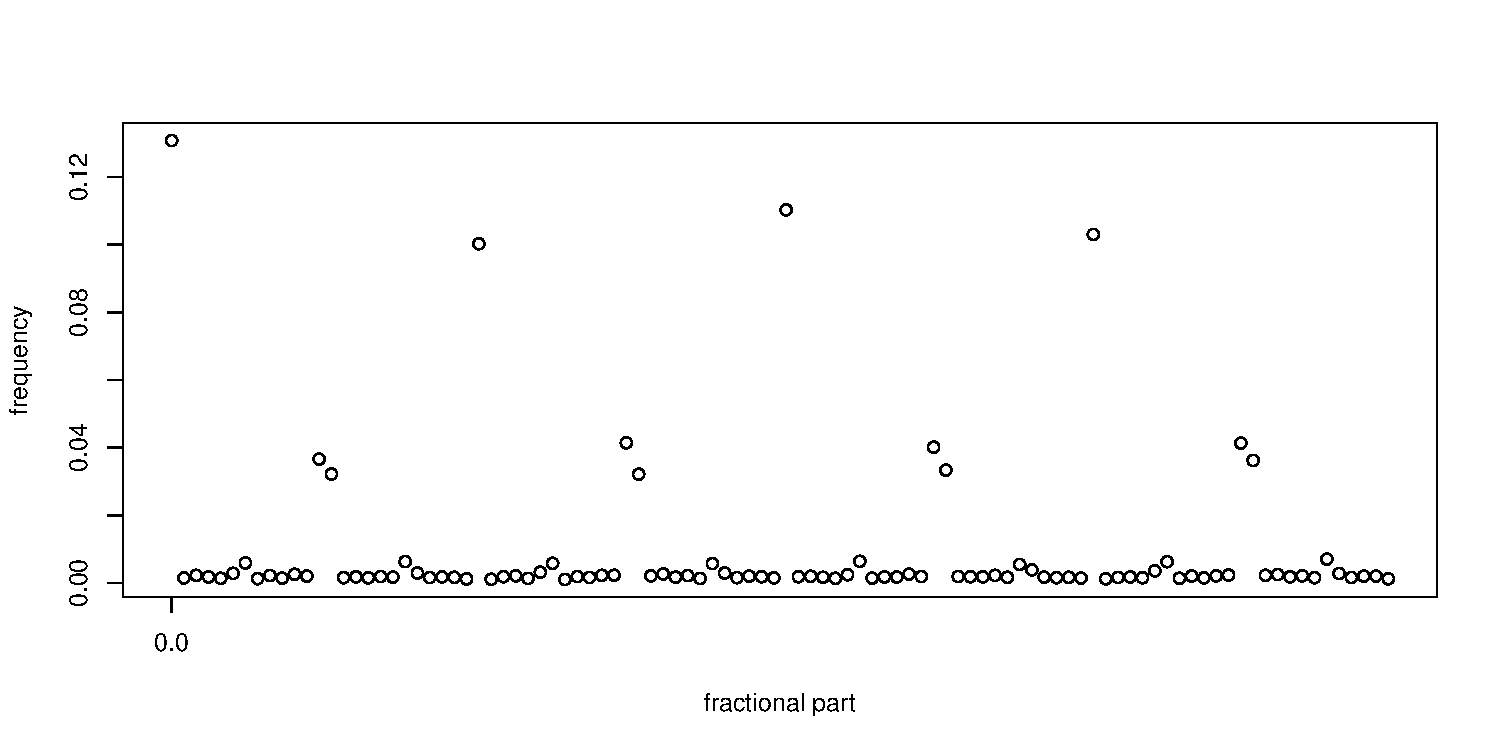
\includegraphics[scale=0.5]{frac.pdf}
	\caption{Frequencies of different fractional values. It can be seen that multiplies of $\frac{1}{4}$ are very frequent. Multiplies of $\frac{1}{8}$ are also common, but they can't be represented exactly using just 2 decimals and they appear in the data using both of the possible roundings.}
	\label{fig:frac}
\end{figure}

\subsection {More complicated models}
We also tried fitting more complicated models to the data.
Simple polynomial fits gave significantly worse results than the first model.
Trying to fit polynomial to the difference data proved difficult as

One possible improvement to the first model we tried was to take average difference
from couple of last stock values. We used this value to predict the next change.
This approach produced few bytes longer codelength than the first model so we
abandoned the idea.
Suprisingly, however, adding a small constant value to the mean location of the normal distribution improved the compressed size by about 1~kilobyte.

Next model we considered was discrete cosine transform.
With low number of coefficients results were clearly worse than from the first model.
With 1000 coefficients theoretical codelength was approximately the same as the first model.

\begin{figure}
\begin{center}
\begin{tabular}{|c|c|}
\hline
    Degree of polynomial & Code length in bits\\ \hline
    0      & 126663 \\  \hline
    1      & 123691 \\ \hline
    2      & 123563 \\ \hline
    3      & 120854 \\ \hline
    4      & 120852 \\ \hline
    5      & 120100 \\ \hline
    6      & 120131 \\ \hline
    30     & 114236 \\ \hline
\end{tabular}
\end{center}
\caption{Code length of first stock using polynomial model}
\label{ex2_polys}
\end{figure}

\section{Task 3}

The third task was to compress shuttle classes using side data that was also available during decompression.
There were 58000 class values to be compressed, each ranging from 1 to 7.
The side data consisted of 9 values for each shuttle class.

The side data didn't contain any duplicates with different classes.
That is, it was possible to create a perfect classifier that detected the class of each item based on just the side data without having to explicitly encode any data besides the classifier.

We created a simple decision tree learner to see how well we could classify the data with a simple tree.
Each node of the decision tree contained a test about whether some element of the side data was smaller than a given value, and each leave contained the class that were most common among the items in the noed.
The learned used the standard decision tree learning technique of choosing the test that maximizes the information gain of the test, which is equal to minimizing the entropy of the resulting two classes.
The algorithm iterates over all possible ways to split the nodes and chooses the best way and recursively advances to split the resulting two sets.

The decision tree learning worked suprisingly well.
It turned out that the tree shown in Figure~\ref{fig:ex3small} with only 4 interior nodes was able to classify the data with precision 99.4379\%.
With 26 interior nodes the tree shown in Figure~\ref{fig:ex3big} was able to perfectly classify the input data.
The tree was so small that it didn't make sense to design any complex compression scheme for it.
Instead we just outputted the tree as C code to minimize the overhead of using the tree.
Thus our final code just read the side data from file and computed the classes using the code generated by the learning algorithm.

The C compiler produced quite a large code for the generated decision tree code, a few hundred bytes.
To reduce this size we changed from generating C code into storing the tree compactly in an array.
The array contains 4 bytes for each internal tree node: 1 byte for indicating each of the two children, 4 bits to indicate the variable to be tested and 12 bits for the value that the variable is compared against.
Thus the total data size of the tree of 26~nodes is just 104~bytes.
The size is so small that it didn't seem sensible to compress it more as any any decompression code would require more space than the saving archieved by compression.

\begin{figure}
    %\begin{center}
	\centerline{\includegraphics[width=1.7\textwidth]{ex3_big.pdf}}
    %\end{center}
    \caption{Exact decision tree}\label{fig:ex3big}
\end{figure}

\begin{figure}
    \begin{center}
	\includegraphics[scale=0.5]{ex3_small.pdf}
    \end{center}
    \caption{Approximate decision tree}\label{fig:ex3small}
\end{figure}

\section{Optimizing the executable size}

As the goal was to minimize total package size, we decided to use C to have as small binary size as possible.
On linux linking to the standard library increases binary size quite a lot, so we avoided using it and implemented input and output in Assembly with system calls instead.




%\bibliographystyle{abbrv}\bibliography{ref}

%\appendix

\end{document}
